\documentclass[10pt]{standalone}
\usepackage[utf8]{inputenc}

\usepackage{./articlethemer}
\usecolortheme{erdiagram}

\usepackage{tikz}
\usetikzlibrary{shapes.multipart}
\usetikzlibrary{matrix}

\tikzset{%
    every matrix/.style={%
        matrix of nodes,%
        anchor=north%
    },%
    layout/.style={%
        row sep=1.5in,%
        column sep=2in,%
    }%
}%

\begin{document}

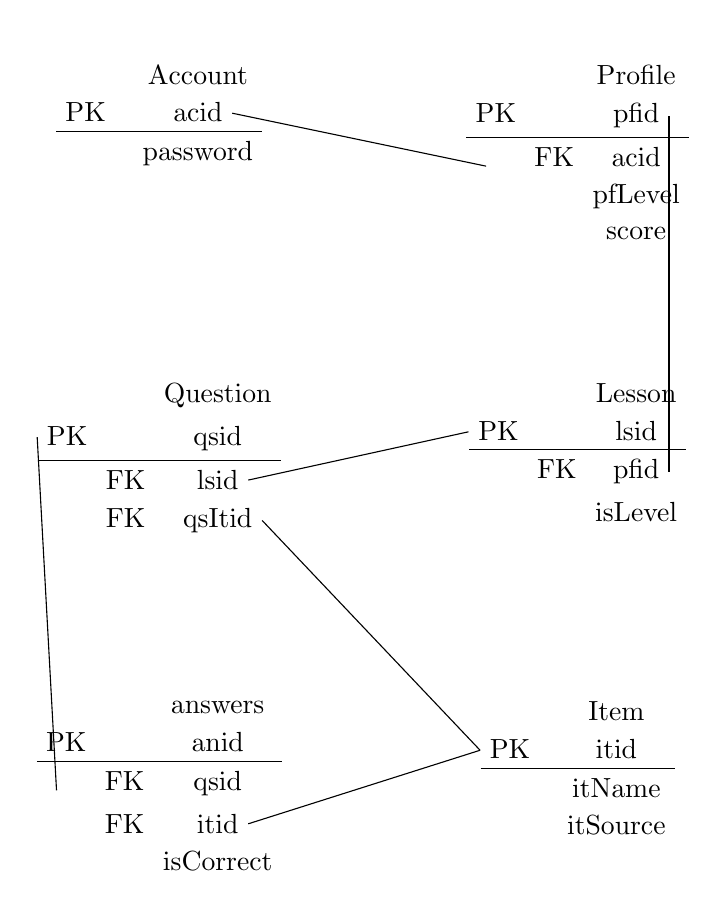
\begin{tikzpicture}
    \matrix[layout] (layout) {
        {} & {} \\
        {} & {} \\
        {} & {} \\
    };
    \matrix (account) at (layout-1-1) {
        {} & {} & Account
        \\
        PK & {} & acid
        \\
        \hline
        {} & {} & password
        \\
    };
    \matrix (profile) at (layout-1-2) {
        {} & {} & Profile
        \\
        PK & {} & pfid
        \\
        \hline
        {} & FK & acid
        \\
        {} & {} & pfLevel
        \\
        {} & {} & score
        \\
    };
    \matrix (lesson) at (layout-2-2) {
        {} & {} & Lesson
        \\
        PK & {} & lsid
        \\
        \hline
        {} & FK & pfid
        \\
        {} & {} & isLevel
        \\
    };
    \matrix (question) at (layout-2-1) {
        {} & {} & Question
        \\
        PK & {} & qsid
        \\
        \hline
        {} & FK & lsid
        \\
        {} & FK & qsItid
        \\
    };
    \matrix (answers) at (layout-3-1) {
        {} & {} & answers
        \\
        PK & {} & anid
        \\
        \hline
        {} & FK & qsid
        \\
        {} & FK & itid
        \\
        {} & {} & isCorrect
        \\
    };
    \matrix (item) at (layout-3-2) {
        {} & {} & Item
        \\
        PK & {} & itid
        \\
        \hline
        {} & {} & itName
        \\
        {} & {} & itSource
        \\
    };
    \draw (account-2-3.east) -- (profile-3-1.west);
    \draw (profile-2-3.east) -- (lesson-3-3.east);
    \draw (lesson-2-1.west) -- (question-3-3.east);
    \draw (question-2-1.west) -- (answers-3-1.west);
    \draw (answers-4-3.east) -- (item-2-1.west);
    \draw (question-4-3.east) -- (item-2-1.west);
\end{tikzpicture}

\end{document}
